\documentclass[11pt]{article}
\usepackage[utf8]{inputenc}
\usepackage[T1]{fontenc}
\usepackage{amsmath,amssymb}
\usepackage{graphicx}
\usepackage{booktabs}
\usepackage{natbib}
\usepackage{authblk}
\usepackage[hidelinks,breaklinks=true]{hyperref}
\usepackage{xurl}
\usepackage{geometry}
\geometry{margin=1in}

\title{\bfseries Ore-Stage Veins at the Sigma Orogenic Gold Deposit Are\\
Spatially Clustered, Not Stress-Shadow Repulsive:\\
a Drill-Core Test, and Why Declustering Fabricates GOE\\
(Val-d'Or, Abitibi, Canada)}

\author[1]{Ruqing Chen}
\affil[1]{GUT Geoservice Inc., Montreal, Quebec, Canada \\ \texttt{ruqing@hotmail.com}}
\date{}

\begin{document}
\maketitle

\begin{abstract}
\noindent
A recurring theme of this research program is the contrast between a single
isolated source and the superposition of many: superposition drives the
consecutive spacing ratio toward the Poisson value, a robust effect. A single
``charge-and-release'' source, however, is a relaxation oscillator whose event
timing is a narrow \emph{scalar clock}, not Wigner--Dyson level repulsion
\citep{chen2026audit}; an earlier reading of orogenic-gold mineralization timing
as GOE ``repulsion'' is corrected to a scalar clock in that audit. Here we test
the \emph{spatial} record of the same deposit class for stress-shadow repulsion ---
stress-shadow repulsion in the spacing of ore-stage veins --- using 235 quartz%
--carbonate vein intercepts logged in four diamond drill holes at the
Archean Sigma orogenic gold deposit (Val-d'Or, Abitibi, Canada; public
assessment report GM~69917). Using a parameter-free spacing-ratio statistic
$\langle r\rangle$ together with the coefficient of variation $\mathrm{CV}$,
and applying \emph{no} declustering preprocessing --- which would act as an
artificial hard core, truncating $P(s\!\to\!0)$ and forcing $\langle r\rangle$
upward toward the GOE value irrespective of the underlying pattern --- we find
that the along-hole
vein spacing is \emph{clustered}, not repulsive: pooled $\langle r\rangle=0.344$
(below the Poisson value $0.386$) and $\mathrm{CV}=1.45$ ($>1$), with a
systematic excess of short spacings. A permutation test gives
$\langle r\rangle_{\rm shuf}=0.33$, indistinguishable from the observed value, so
the clustering is a marginal property of the broad (vein-corridor) spacing
distribution, not a sequential effect. A Kolmogorov--Smirnov test rejects the GOE
(Wigner) hypothesis at $p<10^{-4}$. This result is reproduced by an independent
natural fracture dataset (Lilstock pavement, $\mathrm{CV}=1.52$) and matches
published vein-array statistics ($\mathrm{CV}=1.20$--$1.69$). The same orogenic gold system therefore pairs a \emph{temporal scalar clock} (a
single charge-release source, not level repulsion) with \emph{spatial clustering}
(repeated vein localization on inherited structural weaknesses by crack--seal
cycling, i.e.\ a spatial superposition of many sites). We also document a
methodological hazard:
minimum-separation declustering fabricates spurious GOE statistics from purely
random points, and must not be used to claim spatial repulsion.
\end{abstract}

\section{Introduction}

This program tests how the spacing statistics of geological events depend on
whether one source or many superposed sources are involved: superposition drives
the consecutive spacing ratio toward Poisson \citep{mehta2004}, a robust effect we
rely on below. A single ``charge-and-release'' source was initially read as
producing Gaussian Orthogonal Ensemble (GOE) ``level repulsion'' in the timing of
ore-forming events; a subsequent audit \citep{chen2026audit} shows that such a
source is a relaxation oscillator whose timing is a narrow \emph{scalar clock} ---
a high but shuffle-invariant spacing ratio fixed by the interval coefficient of
variation --- and \emph{not} genuine level repulsion, which requires a chaotic,
strongly-mixed spectrum. We carry that correction here and turn to the spatial
question.

Part~I of the spatial racetrack established that the temporal law has a spatial
analog where an external clock organizes the rock record: cyclostratigraphic
bed spacing, paced astronomically, shows Wigner--Dyson repulsion. The natural
next question is whether \emph{intrinsic} spatial repulsion also exists --- in
particular, whether the stress-shadow mechanism produces regularly spaced veins.
A mode-I (extensional) vein relieves the tensile stress in its neighborhood,
creating a ``stress shadow'' that should suppress the formation of nearby
parallel veins, yielding a minimum spacing and hence repulsion. Orogenic gold
deposits are the ideal natural test: their ore-stage extensional veins are
(i)~mode-I and fluid-overpressure driven, (ii)~chemically distinctive
(quartz--tourmaline--carbonate with bleached alteration selvages), and
(iii)~the spatial counterpart of the temporally clocked ore-forming events.

We test this at the Sigma deposit, a classic Archean orogenic gold system in the
Val-d'Or camp \citep{robert1983}, using a public drill-core dataset. The result
is unambiguous and, for the stress-shadow hypothesis, negative --- but it is
scientifically informative, and we develop its meaning below.

\section{Data and Methods}

\subsection{Dataset}
We use assessment report GM~69917 (Or Integra Quebec Inc., 2016), covering the
Sigma--Lamaque property (NTS 32C/04; Sigma orebody at UTM Zone~18,
$294{,}737$\,E, $5{,}331{,}127$\,N). The report contains complete diamond-drill
logs for four holes: LD-16-001A, SO-16-003, SV-16-009, and SV-16-011. From the
log appendices we extracted every quartz--carbonate vein intercept, recording
its along-hole position, width, mineralogy, and core-axis angle. This yields
235 vein intercepts (Table~\ref{tab:holes}). Because the core-axis angle is not
a true structural attitude (the holes are directional and curved), we do not
attempt orientation-based subsetting; we analyze the full vein population per
hole, which is the most assumption-free test.

\subsection{Statistics}
For each hole we form the sorted sequence of along-hole vein positions and its
spacings $s_i$. We use two parameter-free statistics. The mean adjacent
spacing ratio
\begin{equation}
\langle r\rangle = \left\langle
\frac{\min(s_i,s_{i+1})}{\max(s_i,s_{i+1})}\right\rangle
\end{equation}
takes the value $0.386$ for Poisson (uncorrelated) spacings, $0.536$ for GOE,
and $0.603$ for GUE \citep{atas2013}. It requires no unfolding and is immune to
smooth density gradients. The coefficient of variation $\mathrm{CV}=\sigma_s/
\bar{s}$ equals $1$ for Poisson, exceeds $1$ for clustered point sets, and falls
below $1$ for regular/repulsive sets \citep{cox1966}.

\subsection{No declustering}
Critically, we apply \emph{no} declustering or thinning to the vein positions.
As shown in \S\ref{sec:control}, minimum-separation declustering drives even
purely random point sets toward GOE-like $\langle r\rangle$, and is therefore an
artifact generator. All statistics below are computed on raw vein positions.

\begin{table}[t]
\centering
\caption{Along-hole vein spacing statistics at Sigma. All holes lie in the
clustered regime: $\langle r\rangle$ at or below the Poisson value, and
$\mathrm{CV}\gtrsim 1$. No declustering applied.}
\label{tab:holes}
\begin{tabular}{lrrrr}
\toprule
Drill hole & $n$ & $\langle r\rangle$ & CV & median (m) \\
\midrule
LD-16-001A & 122 & 0.347 & 1.63 & 7.9 \\
SO-16-003  & 53  & 0.367 & 1.17 & 9.5 \\
SV-16-009  & 37  & 0.329 & 1.09 & 5.5 \\
SV-16-011  & 23  & 0.325 & 0.81 & 16.9 \\
\midrule
Pooled     & 235 & 0.344 & 1.45 & 8.9 \\
\midrule
Poisson    &     & 0.386 & 1.00 & \\
GOE        &     & 0.536 & $<1$ & \\
\bottomrule
\end{tabular}
\end{table}

\section{Results}

\subsection{Sigma veins are clustered, not repulsive}
Table~\ref{tab:holes} summarizes the result. Every hole has
$\langle r\rangle \le 0.367$, at or below the Poisson value of $0.386$ and far
from the GOE value of $0.536$. The pooled statistics are
$\langle r\rangle=0.344$ and $\mathrm{CV}=1.45$. A Kolmogorov--Smirnov test of
the normalized spacing distribution against the Wigner (GOE) form is rejected at
$D=0.310$, $p<10^{-4}$; the exponential (Poisson) form is also rejected
($D=0.112$, $p=0.006$) because the data are \emph{more} clustered than Poisson.
A permutation test isolates whether this clustering is a sequential effect or a
property of the spacing distribution alone: shuffling the pooled spacings (which
preserves the marginal distribution but destroys any along-hole order) leaves
$\langle r\rangle$ essentially unchanged, $\langle r\rangle_{\rm shuf}=0.33$
versus $\langle r\rangle_{\rm obs}=0.344$ (difference $+0.02$, within the
shuffle scatter). The low $\langle r\rangle$ is therefore a marginal property of
the broad, high-CV spacing distribution --- the mixture of dense corridors and
sparse intervening rock --- and not a short-range sequential correlation between
neighbouring veins. This is the spatial counterpart of a scalar (marginal)
signal: the pattern is set by where the corridors are, i.e.\ by macroscopic
density structure, rather than by a vein-to-vein spacing rule.
The clustering signature is explicit in the short-spacing fractions: spacings
below $0.1$, $0.2$, and $0.3$ of the mean occur at $19.0\%$, $28.6\%$, and
$35.5\%$, versus the Poisson expectations of $9.5\%$, $18.1\%$, and $25.9\%$
(Fig.~\ref{fig:main}b). There is a consistent excess of closely spaced veins ---
the hallmark of vein corridors, not stress shadows.

One hole (SV-16-011) has $\mathrm{CV}=0.81<1$, a hint of regularity, but with
only 23 intercepts this is not statistically robust and we do not interpret it
as repulsion.

\subsection{Independent corroboration}
The clustering is not a peculiarity of Sigma or of drill-core sampling. We
re-analyzed the Lilstock limestone-pavement fracture network (Bristol Channel,
UK; 350{,}000 mapped fractures), isolating the dominant joint set and computing
the same raw statistics: $\langle r\rangle\approx0.39$, $\mathrm{CV}=1.52$ ---
clustered, identical in character to Sigma. Published calcite vein-array
statistics likewise report $\mathrm{CV}=1.20$--$1.69$ \citep{casoli2026}. Three
independent natural systems --- a drill-cored orogenic gold deposit, a mapped
joint pavement, and literature vein arrays --- all give clustered spacing. Real
fracture and vein systems are clustering-dominated.

\subsection{Methodological control: declustering fabricates GOE}
\label{sec:control}
Earlier in this work an apparent ``GOE'' signal was obtained by applying
minimum-separation declustering (removing points closer than a fraction of the
median spacing). A negative control falsified it: subjecting purely random
(Poisson) points to the same declustering also produces GOE-like
$\langle r\rangle$ (Fig.~\ref{fig:main}d). For the Sigma LD-16-001A hole, raw
$\langle r\rangle=0.347$ rises to $0.44$--$0.50$ under declustering, while random
points rise in lockstep from $0.40$ to $0.54$--$0.61$ --- the two become
indistinguishable. Minimum-separation declustering manufactures regularity from
any input and must never be used to support a spatial-repulsion claim. The
honest diagnostic is the raw $\langle r\rangle$ together with CV.

\begin{figure}[t]
\centering
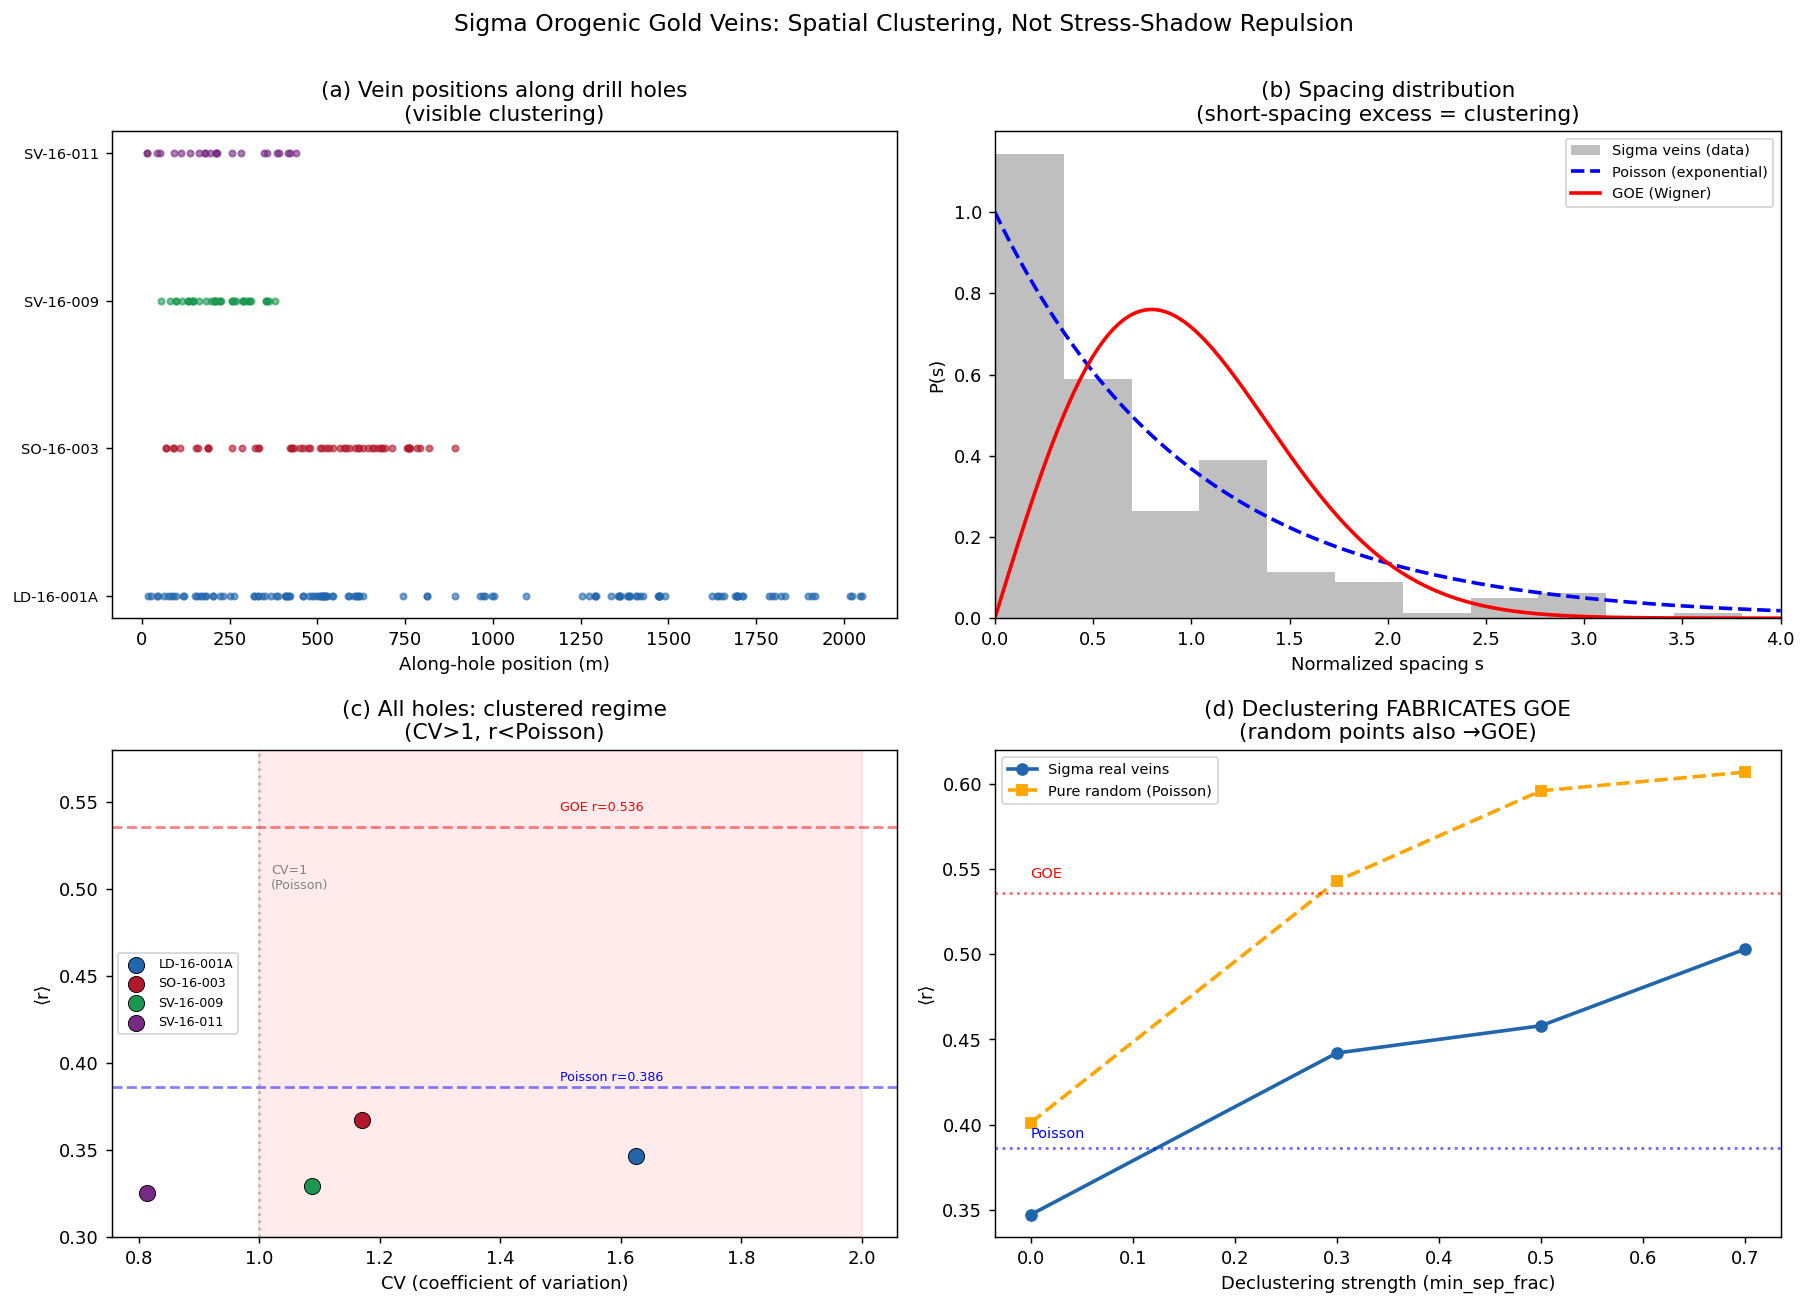
\includegraphics[width=\textwidth]{../figures/sigma_partII_figure.png}
\caption{Spatial statistics of Sigma orogenic gold veins.
(a)~Along-hole vein positions in the four holes; clustering is visible directly.
(b)~Normalized spacing distribution with a short-spacing excess relative to
Poisson (dashed), far from the GOE/Wigner peak (solid).
(c)~All holes occupy the clustered regime ($\mathrm{CV}\gtrsim1$,
$\langle r\rangle\le$ Poisson).
(d)~Declustering fabricates GOE: pure random points (orange) are driven to the
GOE line just as readily as the real veins (blue), proving the artifact.}
\label{fig:main}
\end{figure}

\section{Discussion}

\subsection{A temporal scalar clock with spatial clustering}
The temporal record of orogenic gold mineralization is a scalar charge-release
clock --- a narrow, shuffle-invariant interval distribution, \emph{not} GOE level
repulsion \citep{chen2026audit} --- while the spatial record of the veins is
clustered. Both follow from asking what ``the single source'' produces in each
domain. \emph{In time}, ore-forming pulses are paced by a single deep crustal
process --- episodic fluid overpressure build-up and release in one
fault-valve / metamorphic devolatilization system --- a relaxation oscillator
whose recharge sets a characteristic interval (a refractory period after each
release). This is a \emph{scalar clock}: its spacing ratio is high but carries no
sequential rigidity, and does not amount to level repulsion. \emph{In space},
however, each pulse does not write onto a blank slate: veins nucleate
preferentially on inherited anisotropies (shear-zone fabric, earlier veins,
competent-incompetent contacts), and crack--seal cycling re-opens the same
surfaces repeatedly. The spatial pattern is therefore a \emph{superposition of
many localization sites}, which yields clustering, not repulsion. Geologically,
the negative departure ($\langle r\rangle<0.386$ with $\mathrm{CV}>1$) is the
signature of \emph{fluid channelization}: once a volume is fractured, the damage
zone preferentially focuses subsequent fluid and re-opens to build vein
corridors --- the opposite of stress-shadow exclusion, in which one vein would
suppress the next.

The key conceptual point is that \emph{a single temporal source need not be a
single spatial source}. A temporal scalar clock and spatial clustering coexist in
one system, and the present data show both. Stress-shadow repulsion is real as an
idealized mechanism, but in mature natural systems it is overwhelmed by
structural inheritance and crack--seal localization.

\subsection{Implications}
This refines the program's grand synthesis. The mapping is corrected to
``single isolated relaxation-oscillator source $\rightarrow$ scalar clock (not
GOE); superposition $\rightarrow$ Poisson/clustering'' \citep{chen2026audit}; the
superposition limb is unchanged, and it is the limb that the spatial result here
exercises. For ore systems specifically, the result implies
that vein spacing carries information about structural inheritance rather than
about an instantaneous elastic stress field --- relevant to how vein-density
models are built for exploration.

\subsection{Limitations}
The core-axis angle in the drill logs is not a true attitude, so we did not
attempt to isolate a single structural vein set; it remains possible (though, on
the present evidence and the literature, unlikely) that a chemically and
mechanically pure single-generation extensional set, mapped in outcrop at
centimetre scale, could approach repulsion in a small, localized ore zone. Such
a test requires position-resolved, generation-separated vein maps that are not
available in the public drill record.

\section{Conclusions}
\begin{enumerate}
\item At the Sigma orogenic gold deposit, 235 logged vein intercepts in four
drill holes give pooled $\langle r\rangle=0.344$ and $\mathrm{CV}=1.45$: the
veins are spatially \emph{clustered}, not stress-shadow repulsive. The GOE
hypothesis is rejected at $p<10^{-4}$.
\item The same clustering appears in an independent mapped fracture network
($\mathrm{CV}=1.52$) and in published vein arrays ($\mathrm{CV}=1.20$--$1.69$):
real vein/fracture systems are clustering-dominated.
\item The orogenic gold system pairs a \emph{temporal scalar clock} (a single
charge-release source, not level repulsion \citep{chen2026audit}) with
\emph{spatial clustering} (a superposition of inherited localization sites): a
single temporal source need not be a single spatial source.
\item Minimum-separation declustering fabricates spurious GOE statistics from
random points and must not be used to claim spatial repulsion; the honest
diagnostic is raw $\langle r\rangle$ with CV.
\end{enumerate}

\section*{Changes from version 1 (erratum)}
This is version~2. The spatial analysis is unchanged: the data, the pooled
$\langle r\rangle=0.344$ and $\mathrm{CV}=1.45$ clustering result, the independent
corroboration, all figures, and the demonstration that declustering fabricates
GOE are exactly as in version~1 and stand. The revision concerns only the
\emph{temporal} framing. Version~1 described the timing of orogenic-gold
mineralization as ``temporal level repulsion (GOE)'' and cast the paper as a
``time--space asymmetry.'' A subsequent audit \citep{chen2026audit} shows that a
charge-and-release source is a relaxation oscillator whose timing is a narrow
\emph{scalar clock}: its spacing ratio is high but shuffle-invariant and set by
the interval coefficient of variation, with no spectral rigidity, and the
specific orogenic-gold value is in any case unresolvable given geochronological
age errors. Genuine Wigner--Dyson repulsion requires a chaotic, strongly-mixed
spectrum, which a fluid reservoir does not possess. Accordingly, version~2
reframes the temporal leg as a \emph{temporal scalar clock} (not level repulsion)
and the result as ``temporal scalar clock $+$ spatial clustering'' rather than a
time--space asymmetry. The superposition$\,\to\,$Poisson principle, on which the
spatial argument here rests, is unaffected.

\section*{Data and Code Availability}
All vein-position data (extracted from public report GM~69917) and the analysis
code are provided in the accompanying repository,
\url{https://github.com/Ruqing1963/sigma-spatial-rmt} (version~2.0), archived on
Zenodo. The primary source report is publicly available from the Quebec MRNF
SIGEOM/GESTIM system. The temporal re-audit underlying the version~2 reframing is
in \citet{chen2026audit}.

\begin{thebibliography}{9}
\bibitem[Ata\c{s} et al.(2013)]{atas2013}
Ata\c{s}, Y.Y., et al. (2013).
Distribution of the ratio of consecutive level spacings in random matrix
ensembles. \emph{Phys. Rev. Lett.} 110, 084101.

\bibitem[Casoli et al.(2026)]{casoli2026}
Casoli, E., et al. (2026).
Block-in-matrix deformation and veining at blueschist-facies conditions.
\emph{Geochem. Geophys. Geosyst.}, in press.

\bibitem[Chen(2026)]{chen2026audit}
Chen, R. (2026).
Narrow scalar clocks, not level repulsion: a fourth spurious-GOE hazard and a
re-audit of metallogenic timing statistics. Zenodo,
\url{https://doi.org/10.5281/zenodo.20980670}.

\bibitem[Cox \& Lewis(1966)]{cox1966}
Cox, D.R., \& Lewis, P.A.W. (1966).
\emph{The Statistical Analysis of Series of Events.} Methuen, London.

\bibitem[Mehta(2004)]{mehta2004}
Mehta, M.L. (2004). \emph{Random Matrices}, 3rd ed. Elsevier, Amsterdam.

\bibitem[Robert(1983)]{robert1983}
Robert, F. (1983).
\'Etude du mode de mise en place des veines aurif\`eres de la mine Sigma,
Val-d'Or, Qu\'ebec. Ph.D. thesis, \'Ecole Polytechnique de Montr\'eal, 295 pp.
\end{thebibliography}

\end{document}
